\documentclass{scrartcl}
\usepackage[a4paper,left=1in,right=1in,top=1.2in,bottom=1in]{geometry}
\usepackage{siunitx}
\usepackage{graphicx}
\setkomafont{disposition}{\normalfont\bfseries}
\usepackage{color}
%title
\title{Exercise 05:\\Operating point of a spiking neuron}
\subtitle{Theoretical Neuroscience I}
\author{Maria del Cerro \and Johannes G\"atjen \and Lorena Morton}

%use these for structure/overview
\newcommand\Question{%
  \textbf{Question:}%
}
\newcommand\Answer{%
  \textbf{Answer:}%
}

\begin{document}
\maketitle

In this exercise we simulate a leaky integrate-and-fire neuron with synaptic inputs. Additionally we simulate an identical neuron without a firing mechanism  to determine what the average membrane potential of our neuron would be. Figure \ref{memv} shows the membrane voltage over time for the spiking and the non-spiking neuron with one excitatory and one inhibitory presynaptic neuron. Because the membrane potential never reaches the threshold potential our neuron does not spike and the membrane potential is identical between the spiking and the non-spiking neuron. Only when we increase the excitatory synaptic activation as in Figure \ref{memv_high} do we see a difference between the two neurons.

Next we vary the number of excitatory and inhibitory inputs and observe the resulting output firing rate $\nu_\mathrm{spk}$, as well as the coefficient of variation $c_v$ of the inter-spike interval lengths and the corresponding average membrane potential of the non-spiking neuron $\langle V_\mathrm{ns}\rangle $. The results are summed up in Table \ref{rates}. When we fix the number of inhibitory inputs to zero and only change the number of excitatory inputs, $\langle V_\mathrm{ns}\rangle$ as well as $\nu_\mathrm{spk}$ rise with increasing $N_\mathrm{ex}$, while $c_v$ falls (i.e.\ more regular firing with higher $\langle V_\mathrm{ns}\rangle$). With $N_\mathrm{ex}$ fixed, $c_v$ also falls with rising $\langle V_\mathrm{ns}\rangle$ and $\nu_\mathrm{spk}$, but the differences are smaller than in the first case (less than $0.01$ difference in $c_v$ between 10.3\si{Hz} and 28.7\si{Hz}). Now a higher $N_\mathrm{in}$ produces a lower $\nu_\mathrm{spk}$.

The coefficient of variation is a measure of how regularly a neuron fires. As a rough rule of thumb, one can say, that the higher $\langle V_\mathrm{ns}\rangle$ is, the lower $c_v$ is. This is most clear, when comparing the firing behavior of the neuron for values of $\langle V_\mathrm{ns}\rangle$ a few \si{mV} above the threshold potential of the neuron with the firing behavior when $\langle V_\mathrm{ns}\rangle$ is a few \si{mV} below the threshold potential. In the former case, the ``standard'' behavior for the membrane potential is to rise quickly and reach the threshold potential, where it gets reset. Only when by chance a few more inhibitory than excitatory spikes occur, does the membrane potential not reach the threshold. In the latter case the ``standard'' behavior for the neuron is to maintain a membrane potential below the firing threshold, and it only fires, when by chance the number of excitatory spikes outnumbers the inhibitory spikes by enough. In the latter case spikes are irregular, while in the former case ``non-spikes'' are irregular.

\begin{figure}
\centering
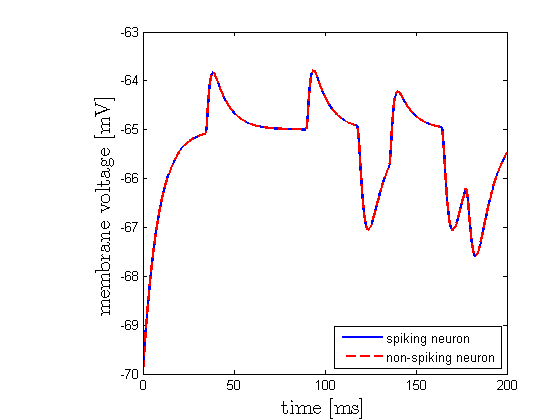
\includegraphics[trim = {2.3cm 0 1cm 0.6cm}, width=0.6\textwidth, clip]{../pics/memv}
\caption{The membrane potential of a LIF neuron with synaptic inputs in blue compared with a non-spiking neuron shown with dashed red. The number of excitatory and inhibitory presynaptic neurons $N_\mathrm{ex}$ and $N_\mathrm{in}$ are both set to one, with the spiking rates $\nu_\mathrm{ex} = \nu_\mathrm{in} = 20\si{Hz}$. Whenever a presynaptic spike occurs the membrane potential increases or decreases a bit, depending on if the presynaptic spike was in the excitatory or the inhibitory neuron, before it relaxes back to the resting potential. Because the threshold potential is never reached the neuron never fires and there is no difference between the spiking and the non-spiking neuron.}
\label{memv}
\end{figure}

\begin{figure}
\centering
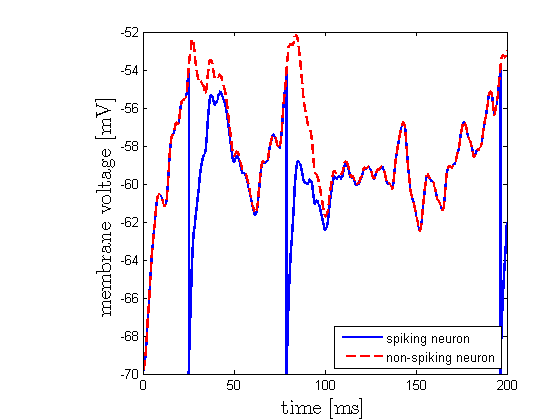
\includegraphics[trim = {2.3cm 0 1cm 0.6cm}, width=0.6\textwidth, clip]{../pics/memv_high_}
\caption{The same setup as in Figure \ref{memv}, but with $N_\mathrm{ex} = 30$. Multiple excitatory spikes in a short amount of time now push the membrane potential above the threshold potential and the spiking neuron fires, whereas the membrane potential of the non-spiking neuron continues to rise. If no spike occurs for some time the two membrane potentials become (almost) equal again.}
\label{memv_high}
\end{figure}

\begin{table}
\centering
\begin{tabular}{c c c c c}
$N_\mathrm{ex}$ & $N_\mathrm{in}$ & $\nu_\mathrm{spk} [\si{\hertz}]$ &$\langle V_\mathrm{ns}\rangle [\si{mV}]$ & $c_v$ \\ \hline \hline
30 & 0 & 10.53 & -57.35 & 0.86\\
40 & 0 & 30.27 & -55.17 & 0.70\\
56 & 0 & 69.13 & -51.98 & 0.53\\ \hline
100 & 30 & 10.33 & -61.33& 0.953\\
100 & 22 & 28.7 & -58.62& 0.946\\
100 & 13 & 70 & -54.55& 0.833\\
\end{tabular}
\caption{Number of excitatory presynaptic neurons $N_\mathrm{ex}$, Number of inhibitory presynaptic neurons $N_\mathrm{in}$, output spiking rate $\nu_\mathrm{spk}$, average non-spiking membrane potential $\langle V_\mathrm{ns}\rangle$ and coefficient of variation of the inter-spike interval lengths $c_v$. In the top part $N_\mathrm{in}$ was fixed to zero and $N_\mathrm{ex}$ was varied, in the bottom part $N_\mathrm{ex}$ was fixed to 100 and $N_\mathrm{in}$ was varied.}
\label{rates}
\end{table}

\subsection*{Operating point}

To determine the operating point of the neuron, we fix $N_\mathrm{ex}=100$ and vary $N_\mathrm{in}$ to find the maximum value of $c_v$. Figure \ref{cv_aveV} shows a plot of $c_v$ as a function of $\langle V_\mathrm{ns}\rangle$. $c_v$ decreases linearly for values of $\langle V_\mathrm{ns}\rangle > -58\si{mV}$ but for smaller values of $\langle V_\mathrm{ns}\rangle$ the data does not show a clear relation, as the values for $c_v$ fluctuate strongly. Nevertheless, $c_v$ appears to fall with smaller values of $\langle V_\mathrm{ns}\rangle$. As such, the operating point of the neuron can be estimated to be around $-58\si{mV}$, or $4\si{mV}$ below the threshold potential of $-54\si{mV}$.

\begin{figure}
\centering
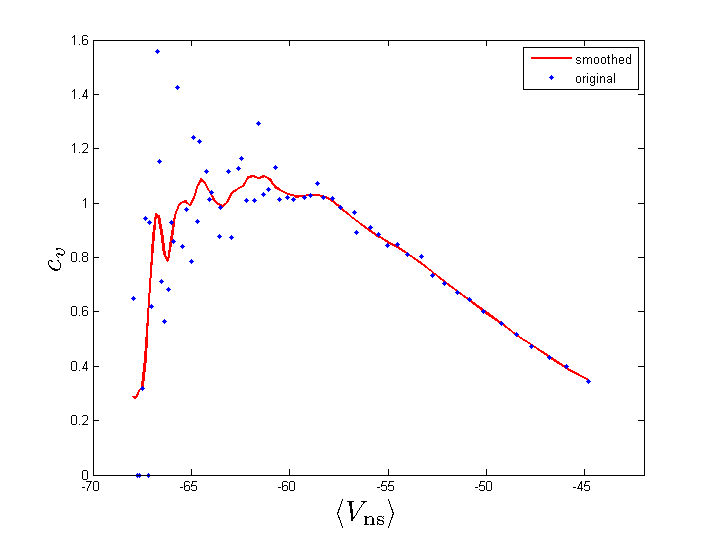
\includegraphics[trim = {1.2cm 0 1cm 0.6cm}, width=0.8\textwidth, clip]{../pics/cv_aveV}
\caption{$c_v$ as a function of $\langle V_\mathrm{ns}\rangle$  for $N_\mathrm{ex}=100$ and varying $N_\mathrm{in}$. The original data is shown with blue points, and smoothed data is shown with the red line.}
\label{cv_aveV}
\end{figure}


%include picture
%\begin{figure}
%\centering
%\includegraphics[trim = {1.3cm 0 2cm 0.9cm}, width=\textwidth, clip]{../pics/picname}
%\caption{caption text}
%\label{label}
%\end{figure}
\end{document}